\section{Force calculation - potentials}
\label{sec:md_forces}
In general, the potential energy is given as a function of the configuration given by the atom positions
\begin{align}
	U(\vec{r}) = \sum_{i<j}U_2(r_{ij}) + \sum_{i<j<k} U_r(\vec r_i, \vec r_j, \vec r_k) + ...,
\end{align}
where $\vec r$ is the phase space point, $U_n$ is a function of the positions of $n$ atoms, $r_{ij}$ is the relative distance between atom $i$ and $j$, $\vec r_i$ is the position of atom $i$. Advanced potentials such as ReaxFF can even have 5-atom contributions to the energy\cite{van2001reaxff}. The reason for this is simple; when three atoms are close to each other, the electron configuration might be different than if there were only two atoms. These effects play a large role in forming molecules, such as water. Numerically, the calculation of forces is the most expensive part of the whole program, so for simple systems or educationally purposes it might be sufficient to use the Lennard-Jones potential.
\subsection{The Lennard-Jones potential}
We often see this potential referred to as the 6-12 potential, due to its functional form. It is a function that inherently carries the two main properties of atomic forces; the short-ranged Pauli repulsion and the long-ranged van der Waals force. The potential is only between pairs of atoms
\begin{align}
	\label{eq:md_potential_energy}
	U_{LJ}(r_{ij}) = 4\epsilon\left[\left(\frac{\sigma}{r_{ij}}\right)^{12} - \left(\frac{\sigma}{r_{ij}}\right)^{6}\right],
\end{align}
where $r_{ij}$ is the relative distance between atom $i$ and $j$, $\epsilon$ and $\sigma$ are coupling constants giving the depth of the potential well and the distance where the potential is zero. The force is given as the gradient of this potential yielding 
\begin{align}
	\label{eq:md_lj_force}
	\vec F_{LJ}(\vec{r_{ij}}) = -\nabla U_{LJ}(r_{ij}) = -24\epsilon\left[2\left(\frac{\sigma^{12}}{r_{ij}^{13}}\right) - \left(\frac{\sigma^6}{r_{ij}^7}\right)\right]\vec u_{ij},
\end{align}
where $\vec u_{ij}$ is the unit vector pointing from atom $i$ to atom $j$. In this thesis, we will only study the LJ-potential, so we simplify the notation by choosing $\vec F_{LJ} = \vec F$ and $U_{LJ} = U$. The form of the potential is shown in figure \ref{fig:md_lennard_jones}.
\begin{figure}[h]
\begin{center}
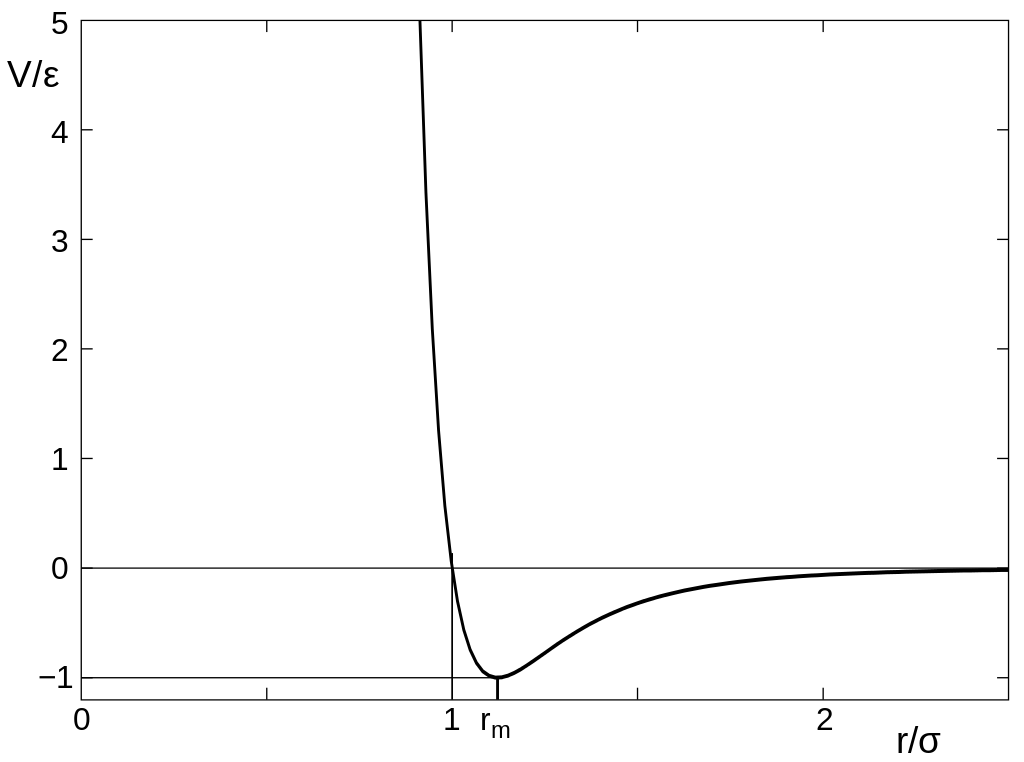
\includegraphics[width=0.8\textwidth, trim=0cm 0cm 0cm 0cm, clip]{MD/figures/lennard_jones.png}
\end{center}
\caption{The Lennard-Jones potential as a function of relative distance $r_{ij}$ between two atoms. (Image from \url{http://en.wikipedia.org/wiki/File:12-6-Lennard-Jones-Potential.svg}, accessed 18 March, 2014.)}
\label{fig:md_lennard_jones}
\end{figure}
With this potential, we can in principle calculate the forces between atoms that are 10 meters apart. We already know the answer though, it should be very, very close to zero. Atoms being far away from each other do not interact. This distance is actually not very large. If we insert $r_{ij} = 3.0\sigma$ into equation \eqref{eq:md_lj_force}, and choose units so that $\sigma = \epsilon = 1.0$, we get $F(r=3.0) \approx 0.01$ (compared to the maximum attraction near the potential well $F(r = 1.24) \approx 2.4$, more than 100 times larger). The force decreases slowly towards zero for larger displacements. We can exploit this property and only compute forces between atoms displaced by a distance smaller than some cut-off radius.
\subsection{Cut-off radius}
\label{sec:md_implementation_two_body_forces}
In principle, we have to sum over all pairs in the system which for $N$ atoms is $O(N^2)$. This calculation can be reduced to $O(N)$ by realizing that the gradient of the potential (hence the force) is nearly zero at $r \approx 3.0\sigma$. We now introduce the cut-off radius $r_\text{cut}$, which we choose to be $r_\text{cut} = 3.0\sigma$. The force between a pair of atoms $F(r_{ij})$ is then written as
\begin{align}
	\vec F(\vec r_{ij}) = \left\{
	\begin{array}{l l}
		-24\epsilon\left[2\left(\frac{\sigma^{12}}{r_{ij}^{13}}\right) - \left(\frac{\sigma^6}{r_{ij}^7}\right)\right]\vec u_{ij} & \text{if } r_{ij} \leq r_\text{cut}\\
		0 & \text{if } r_{ij} > r_\text{cut}.
	\end{array}\right .
\end{align}
This means that we don't have to compute the forces between atoms that are more than $r_\text{cut}$ apart. So \textit{locally}, within this radius $r_\text{cut}$, the number of pairs we need to sum over is proportional to $\rho_n^2$, but if we double the system size, most of the extra atoms do not feel the forces from the atoms already in the system since they are separated by more than $r_\text{cut}$. So the calculation of forces is $O(N)$.